\section{Setup}
The experiment written in Python in form of a Jupyter Notebook. At first the function for providing the optimal pool size was implemented, the exact implementation can range from Bernoulli experiment to another form. When the optimal pool size is found, which is the second research question where I created 10000 objects and assign them to a certain pool and assign them a corruption rate ranging from 0.01 to 0.2. The corruption rate is the base for the Bernoulli experiment. After object creation, the objects are ingested into the archive, during this process each pool is persisted on the blockchain. This happens in an interaction between a python client and a local installation of the Ethereum blockchain. Ganache is used for local development on the Ethereum side and pythons Web3 is used as a client. While ingesting and uploading onto the blockchain I will monitor the amount of gas used and the exact number of write transactions. The more exact method of monitoring the operation cost is by adding up the gas cost, since gas can be transformed into ETH. The first measurement will be theoretical and the second empirical where I monitor the amount of ETH available for the experiment account. e.g. if I start the experiment with 100 ETH and at the end I have 90 ETH left the operation cost was 10 ETH. If the experiment local is successful I will deploy the smart contract on the Ropsten testnet and add time measurement to the process since the blockchain is now real and distributed on the network. I expect the time needed to ingest and upload on the blockchain to increase the cost should stay the same. When the objects are ingested into the dummy archive and the pools are uploaded onto the blockchain I will retrieve random samples from the original set of objects and check if they are corrupt, maybe I will assign corruption at random to this random sample, and then I have to implement a repair function, this function also affect the operation cost, since when a corrupted file is found the whole pool has to be re-computed resulting in pool size + 1 local transactions and one blockchain write transaction. In the retrieval process I will monitor the time and nullify the cost since read operations on the blockchain are free of charge, nonetheless I will count the number of transactions needed for the process. After retrieval and repairing the pools I will look into the number of transactions needed, and the time needed for the whole process. The result will be one row of a table and the experiment can be redone with different pool sizes or corruption rates to get a nice table with descriptive statistics. 
At last, I will split the objects and metadata and adapt the corruptions rates and redo the whole experiment and compare the results. 
\section{Object Identity}
When and where should the pool ID be stored, there are possibilities that the pool ID is assigned with pool creation, but that would mean that I have to update the object which is supposed to preserve, should the pool ID be in the metadata of the object= if no, where should we store the link between the object and its respective pool. It is easy to keep the links in the local Jupyter notebook but in an industrial environment keeping those links is rather hard. For now, I keep the transaction hash with the pool object.
\section{Object}
An object in this experiment is simply a SHA256 value, since the preservation process does not care if a picture, text or video is secured by the hash. An object also holds the reference to its pool, where in a real case the poolId is stored in the object's metadata. For the sake of the experiment, the initial bulk is numbered from 1 to N, where the SHA256 value is then assigned to the object. An object also has a float value which indicates the chance of it of being corrupted, this value is used in the Bernoulli experiment to determine the optimal pool size based on the corruption rate of all objects. The final member variable of the object is a boolean flag which indicates whether an object is corrupted or not.

\section{Pool}
A pool in this experiment is a collection of objects with size k. The root hash of a pool is a hash-list of every object in the pool.
\section{Archive Mock}
For the sake of the experiment I will mock the functions of a digital archive in python with the following relevant functions implemented: (1) $bulk_ingest$ (2) retrieve (3) $get_objects_by_poolId$ (4) repair. (1) Is for ingesting a bulk of objects with their respective metadata, it is expected that the poolId is already set for the object. The bulk itself does not know anything about the pool sizes or the amount of pools. The archive therefore is independent of the implementation of a pool and only need to know the poolId of an object. The poolId may be stored in the Preservation Description Information of an object \cite{lee2010open}. (2) Retrieve a single object from the archive. (3) The implementation of this function in a real digital archive may vary from my implementation, where I return all objects stored in the archive with matching poolId. This function is here to provide information regarding the original objects of a pool, this is necessary to rebuild the pool and recalculate the pool hash for someone who might want to check whether an object in the archive got corrupted. (4) The function which handles the case when a corrupted pool was found. It is a costly function where one write transaction to the blockchain and additional data scrubbing has to be made. When a pool is found to be corrupted, each object in the pool is suspected to be corrupted too and therefore each object has to be replaced by a copy and reassembled in a pool, which hash is then again persisted on the blockchain.
The mock also provides a function to simulate corruption, where each object in the archive has a chance to corrupt itself.
\section{Program Flow}
During development, I have seen that the pool size should not be too high.
When a corrupted pool is found, make sure to not double write the same pool to the blockchain
You even got an advantage when you repair objects, since you have to scrub each object in the pool with a fresh copy.
\section{Dataset}\label{sec:dataset}
I analyzed the format-corpus\footnote{\url{https://github.com/openpreserve/format-corpus}} from Open Preserve Foundation\footnote{\url{ http://openpreservation.org/}} to get a better understanding of various file formats, mostly on how volatile they are. The latest commit for my analysis was \textit{commit 4e4b9a34540f72612ba6eab2d28bccceb7a848ae}\footnote{\url{https://github.com/openpreserve/format-corpus/commit/4e4b9a34540f72612ba6eab2d28bccceb7a848ae}} on the 16th of February. The format-corpus is well-structured in a public GitHub repo with a decent amount of reputation in form of GitHub stars, where other datasets did provide corrupt links;were not available or did expect a tedious amount of time to download and re-structure them. Convenience; diversity of file extensions; and reputation of the organization affected my decision to use the format-corpus for analysis.
For the analysis I used the python package folderstats\footnote{\url{https://pypi.org/project/folderstats/}} which transforms a directory into a pandas\footnote{\url{https://pandas.pydata.org/}} dataframe. The repository contains 1560 files with 90 distinct file extensions, e.g. 986 \textit{.xml} files which are mostly PRONOM\footnote{\url{https://www.nationalarchives.gov.uk/PRONOM/}} registry files or \textit{pom.xml} files in case of java projects. In Figure \ref{fig:extension_distribution} you can see the distribution of file extensions where \textit{.xml} files make 62.2 percent of the portion and PDF with 6.79 percent as the second-largest portion.
\begin{figure}[h]
    \caption{Distribution of file extensions in the format-corpus of Open Preserve Foundation. \url{https://github.com/openpreserve/format-corpus}}
    \label{fig:extension_distribution}
    \centering
    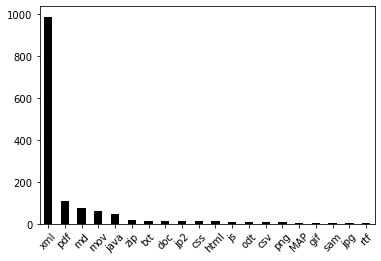
\includegraphics[width=0.5\textwidth]{extension_distribution.png}
\end{figure}

\subsection{Transformations}
To get a baseline estimate on how volatile certain extensions are due to updates and alterations, I analyzed Git logs and count how many times a file extension was involved in a commit. The resulting column \textit{positives} was always higher or equal than the occurrence of a file extension, since each file was involved in at least one commit, the initial commit of the file. To count the commits I used the python package gitphyton\footnote{\url{https://gitpython.readthedocs.io/en/stable/}} and utilized the git command --log. For each file in the repository, I fired up the command \textit{git log --oneline filename} in python which resulted in one or multiple lines of logs. Latter I used the multiline log as an input for the \textit{.splitlines()} function which results in an array of log lines, the length of this array minus 1 (the initial commit) is used to determine the new column \textit{positives} in the dataframe which shows if and how often a certain file has changed over the lifetime of the git repository. 
This method of determining the volatility of a certain file extension is by no means ideal, but there is no other method to look into how often a certain file has changed without monitoring them on a system for a certain time interval. Therefore, I have decided to use the amount of file alterations in the git repository as a rough estimate.
The estimated prevalence rate $p$ of a file extension is calculated with $positives/N$, see Table \ref{tb:git-alterations}
\begin{table}[ht]
    \caption{Volatility of certain file extensions in the format-corpus dataset}
    \centering
    \begin{tabular}{ c c c c c}
    \label{tb:git-alterations}
     extension & N & positives & p & k\\ 
     \hline
     XML & 986 & 432 & 0.43  & 2\\  
     \hline
     PDF &106 &2 &0.01  & 8\\
     \hline
     MD & 74 & 17 & 0.22  & 3\\    
     \hline
     MOV&61 & 0 & 0.00 &  61\\  
     \hline
     JAVA &47 &39&0.82 & 2 \\  
     \hline
     ZIP & 17 &0 &0.00 &  17\\
     \hline
     TXT & 14 & 2 & 0.14 &  4\\ 
     \hline
     DOC & 13 & 0 & 0.00 &  13\\   
     \hline
     JP2 & 12 & 0 & 0.00 &  12\\    
     \hline
     HTML & 11 & 6 & 0.54 &  2\\   
     \hline
     CSS & 11 & 4 & 0.36 & 2 \\ 
     \hline
     JS & 10 & 3 & 0.3 & 3
    \end{tabular}
\end{table}
I applied Equation \ref{eq:simple_poolsize}, created by \cite{regen2020simple}, to each row in Table \ref{tb:git-alterations} to calculate the optimal pool size for each file extension.
\begin{equation}\label{eq:simple_poolsize}
    k = 1.24* (positives/N)^-0.466
\end{equation}

\section{Wrap up}
In this Chapter, I have presented the environment and dataset needed in order to answer the research questions which are presented in Chapter \ref{ch:evaluation}
TODO weiterarbeiten